\documentclass{article}

\usepackage[utf8]{inputenc}
\usepackage[T1]{fontenc}
\usepackage[greek,english]{babel}
\usepackage{alphabeta}
\usepackage{amsmath}
\usepackage{amssymb}
\usepackage{graphicx}
\usepackage{subcaption}
\usepackage{epstopdf}
\usepackage[margin=1in, paperwidth=8.3in,paperheight=11.7in]{geometry}
\usepackage{hyperref}
\usepackage{paracol}

\newcommand\course{ΗΡΥ 411}
\newcommand\courseName{Ενσωματωμένα Συστήματα Μικροεπεξεργατών}
\newcommand\semester{Χειμερινό 2020-2021}
\newcommand\assignmentNumber{Εργαστήριο 7-8}
\newcommand\studentName{Μαυρογιώργης Δημήτρης}                           
\newcommand\studentNumber{2016030016}

\title{\underline{\textbf{\assignmentNumber}}} 
\author{\textsc{\textbf{Όνομα:}}  \studentName\\
		\textsc{\textbf{ΑΜ:}}  \studentNumber\\
		\course \ - \courseName\\ 
		\textsc{Πολυτεχνείο Κρήτης}
		}
\date{\today}
\begin{document}
	\maketitle

\section*{Σκοπός}
	Σκοπός του έβδομου και όγδοου εργαστηρίου είναι να δημιουργήσουμε ένα απλό δρομολογητή με μικρή πολυπλοκότητα. Γι' αυτό το λόγο δημιουργήθηκαν τρεις απλές ρουτίνες οι οποίες κάνουν κάποιες αλλαγές στο PORTA. Επιπλέον, στο κυρίως πρόγραμμα, αντί να έχουμε ένα κενό while loop, κάνουμε κάποιους ελέγχουν για να δουμε πια ρουτίνα εκτελείται και ποια είναι η επόμενη, ώστε να κάνουμε το context switching μεταξύ αυτών των διεργασιών.

\section*{Περιγραφή της υλοποίησης}
	Αρχικά, έγιναν κάποια define των χαρακτήρων της κάθε εντολής, προκειμένου να γίνουν οι έλεγχου στον interrupt handler της USART ότι ήρθε σωστά η εντολή. Επίσης, δηλώθηκαν κάποια flag τα οποία ενεργοποιούν ή απενεργοποιούν οι TIMER0 και TIMER1, ενώ δεσμεύτηκε και χώρος στη μνήμη που αποθηκεύουμε κατα το context switch τα δεδομένα του PORTA για κάθε διεργασία ξεχωριστά. Επίσης, δηλώθηκαν και ένα array για τα enables των διεργασιών και ένα βοηθητικό byte στο οποίο αποθηκεύονται τα enable που λαμβάνονται από τη USART.\\
	
	\noindent
	Πιο συγκεκριμένα, όσον αφορά την υλοποίηση, από τα προηγούμενα εργαστήρια έχουμε κρατήσει αυτούσια την αρχικοποίηση του timer0 με σκοπό να αφήνουμε την κάθε διεργασία να αλλάζει το PORTA κάθε 1ms και να μην γίνονται πολλές αλλαγές σε πολύ μικρό αριθμό κύκλων. Eπιπλέον, από το προηγούμενο εργαστήριο χρησιμοποιήθηκαν αυτούσιες οι ρουτίνες για receive και transmit από τη σειριακή θύρα, καθώς και η αρχικοποίηση του USART.\\
	
	\noindent
	Παράλληλα, για την υλοποίηση του timeslice των 100ms, χρησιμοποιήθηκε ο timer1. Για την αρχικοποίησή του ορίζουμε στον καταχωρητή TCCR1B prescaler 64, ενεργοποιούμε στον TIMSK τo OVF interrupt του timer1 (bit TOIE1), ενώ αρχικοποιούμε τον 16-bit καταχωρητή TCNT1 με την τιμή 0xC2F6, η οποία προκύπτει ως εξής: 
	$$ TCNT1 = MAX\_VAL - \frac{DELAY*FREQ}{PRESCALE} = 65535 - \frac{100 ms * 10 MHz}{64} = 49910$$
	
	\noindent
	Στη συνέχεια, δημιουργήθηκε και μια βοηθητική συνάρτηση, η οποία ελέγχει αν αλλαξε κάποιο από τα enable bits στη global μεταβλητή func\_enable ο USART handler και ανάλογα θέτει TRUE ή FALSE στην κατάλληλη θέση του array func\_num. Mε αυτό τον τρόπο, εξασφαλίζουμε ότι μια διεργασία δε θα τελειώσει πρόωρα, δίχως να κάνει context switch με την επόμενη στη σειρά.
	 
	\pagebreak
	\begin{figure}[h!]
		\centering
		\begin{subfigure}[t]{0.5\textwidth}
			\centering
			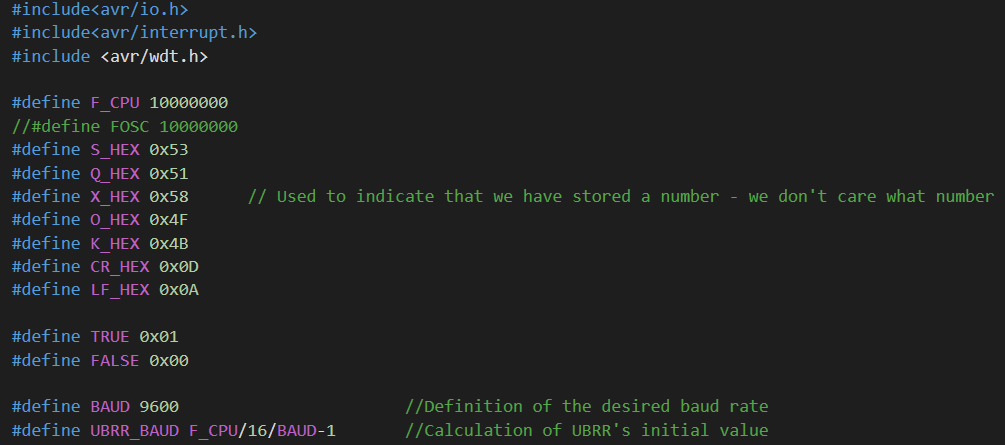
\includegraphics[height=3cm, width=\linewidth]{./results/lab8_defines.png}
			\caption{C code for defines}
		\end{subfigure}%
		~
		\begin{subfigure}[t]{0.5\textwidth}
			\centering
			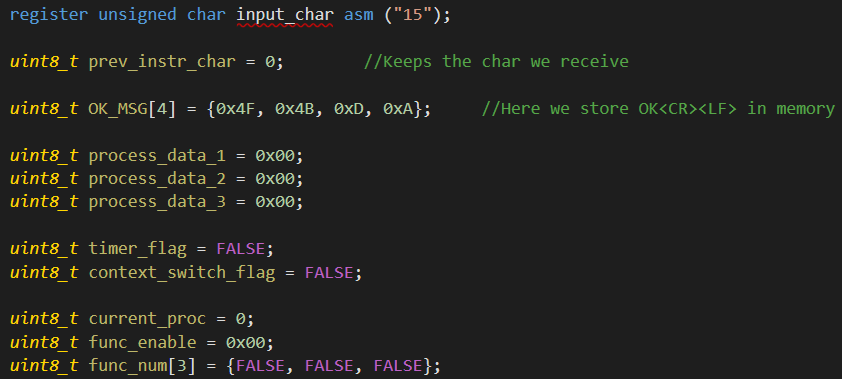
\includegraphics[height=3cm, width=\linewidth]{./results/lab8_global_variables.png}
			\caption{C code for declaring global variables}
		\end{subfigure}
		
		\begin{subfigure}[t]{0.5\textwidth}
			\centering
			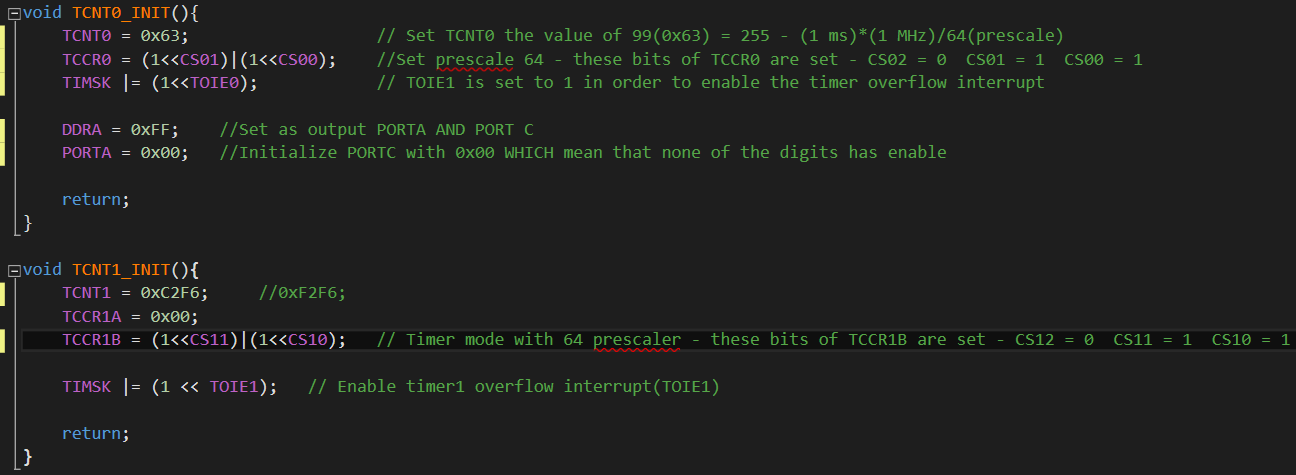
\includegraphics[height=3cm, width=\linewidth]{./results/lab8_timers.png}
			\caption{C code for TIME0/TIMER1 initiliazation}
		\end{subfigure}%
		~
		\begin{subfigure}[t]{0.5\textwidth}
			\centering
			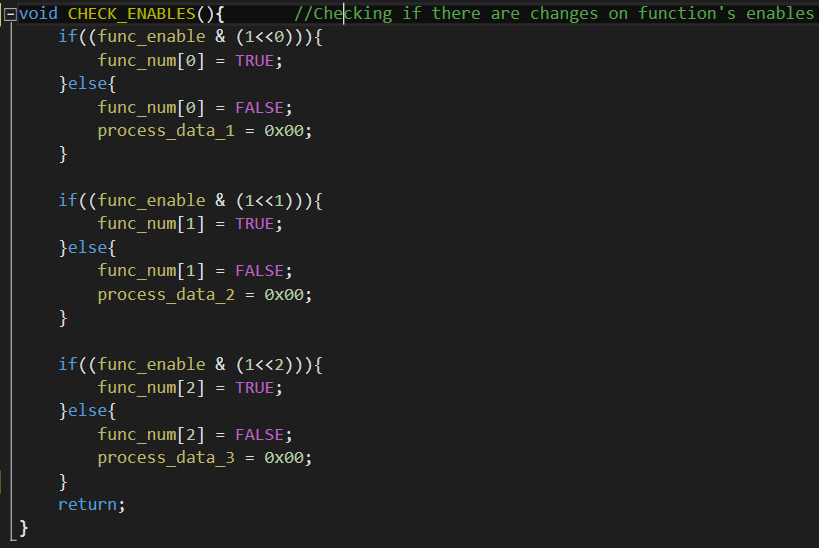
\includegraphics[height=3cm, width=\linewidth]{./results/lab8_enables.png}
			\caption{C code for checking new function enables}
		\end{subfigure}	
	\end{figure}
	
	\noindent
	Όσον αφορά τις τρεις διεργασίες, η πρώτη διεργασία κάνει την εναλλαγή του PORTA από "10101010" σε " 01010101", η δεύτερη διεργασία είναι μια απλή υλοποίηση ενός ring counter, ενώ η τρίτη και τελευταία διεργασία είναι η υλοποίηση ενός μετρητή που μετρά από το "0x00" ως το "0xFF".  \\
	\begin{figure}[h!]
		\centering
		\begin{subfigure}[t]{0.5\textwidth}
			\centering
			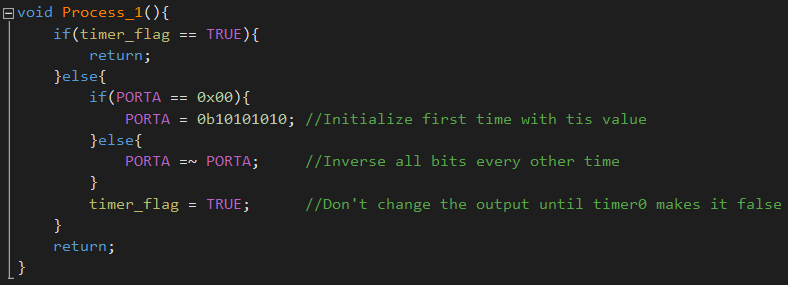
\includegraphics[height=3.5cm, width=\linewidth]{./results/lab8_proc_1.png}
			\caption{C code for Process 1}
		\end{subfigure}%
		~
		\begin{subfigure}[t]{0.5\textwidth}
			\centering
			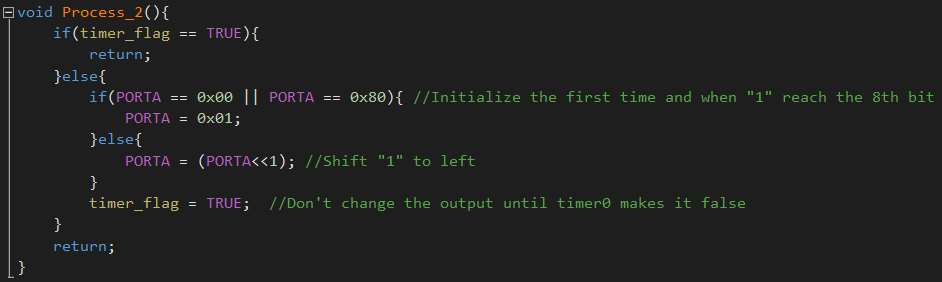
\includegraphics[height=3.5cm, width=\linewidth]{./results/lab8_proc_2.png}
			\caption{C code for Process 2}
		\end{subfigure}
	
		\begin{subfigure}[t]{0.5\textwidth}
			\centering
			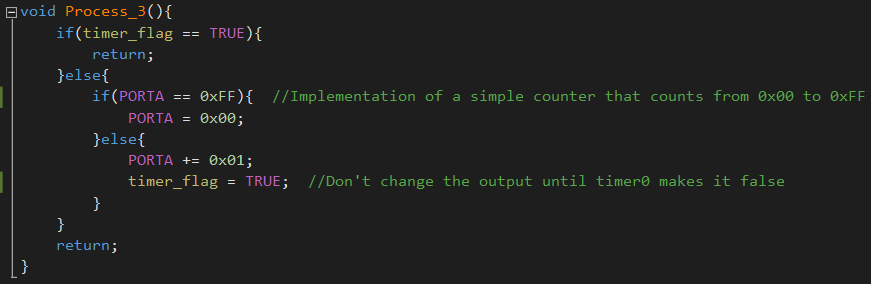
\includegraphics[height=3.5cm, width=\linewidth]{./results/lab8_proc_3.png}
			\caption{C code for Process 3}
		\end{subfigure}
	\end{figure}
	
	\noindent
	Στο κυρίως πρόγραμμα πέρα από τα initialize των timers και usart, έχουμε ένα loop στο οποίο αρχικά ελέγχουμε αν έχει έρθει κάποια διεργασία από τις τρεις για πρώτη φορά. Σε αυτή την περίπτωση, όποια διεργασία έρθει πρώτη την θεωρούμε ως current process.\\
	
	\noindent
	Στη συνέχεια, αν είναι ενεργοποιημένη κάποια ρουτίνα, την εκτελούμε και ελέγχουμε αν έχει τελειώσει το timeslice των 100ms. Στην περίπτωση που έχει τελειώσει, ελέγχουμε για κάποια αλλαγή στα enables και αναλόγως πηγαίνουμε στην επόμενη. Αν πχ είμαστε στο Process 1 και είναι απενεργοποιημένη η 2 και ενεργοποιημένη η 3, τότε η επόμενη στη σειρά είναι η 3 οπότε κάνουμε context switch μεταξύ της 1 και της 3 παραλείποντας την 2. Συνεπώς, μέσα στο while loop ελέγχουμε όλους τους πιθανούς συνδυασμούς για το ποια είναι ενεργοποιημένη και ποια απενεργοποιημένη και αναλόγως κάνουμε το contex switch.
	
	\begin{figure}[h!]
		\centering
		\begin{subfigure}[t]{0.5\textwidth}
			\centering
			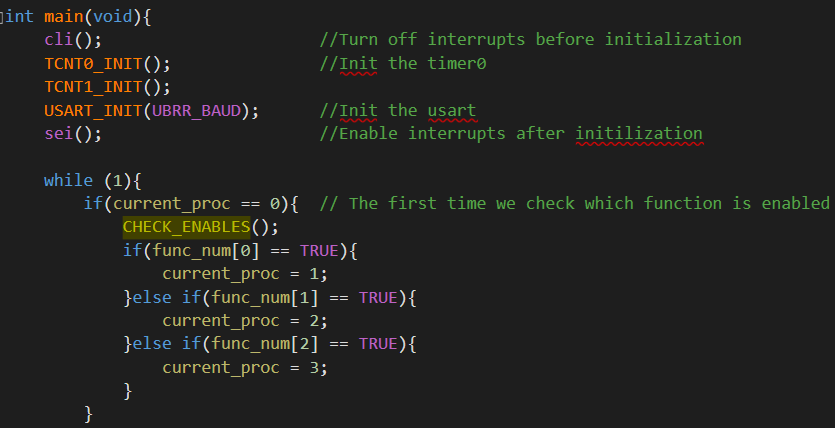
\includegraphics[height=3.5cm, width=\linewidth]{./results/lab8_main_init.png}
			\caption{C code for main initialization}
		\end{subfigure}%
		~
		\begin{subfigure}[t]{0.5\textwidth}
			\centering
			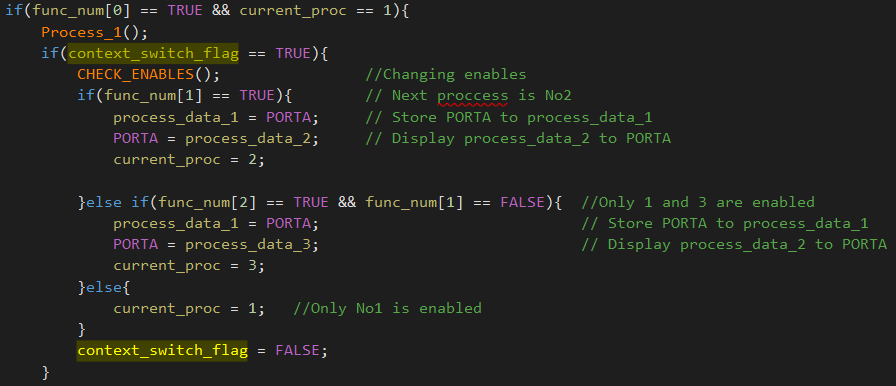
\includegraphics[height=3.5cm, width=\linewidth]{./results/lab8_main_proc_1.png}
			\caption{C code for Process 1 context switching}
		\end{subfigure}
	
		\begin{subfigure}[t]{0.5\textwidth}
			\centering
			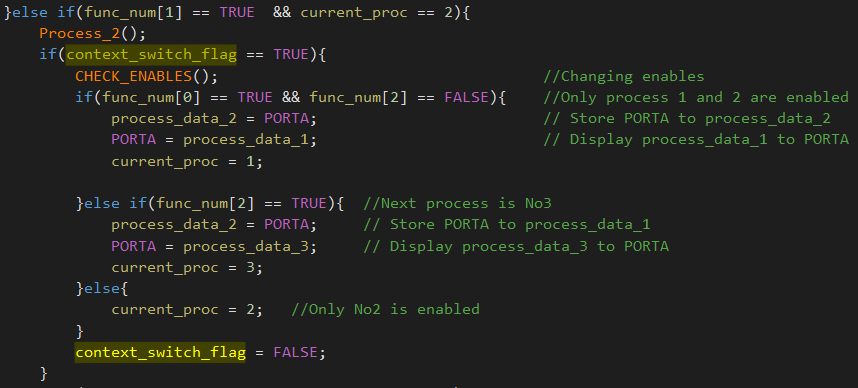
\includegraphics[height=3.5cm, width=\linewidth]{./results/lab8_main_proc_2.png}
			\caption{C code for Process 2 context switching}
		\end{subfigure}%
		~	
		\begin{subfigure}[t]{0.5\textwidth}
			\centering
			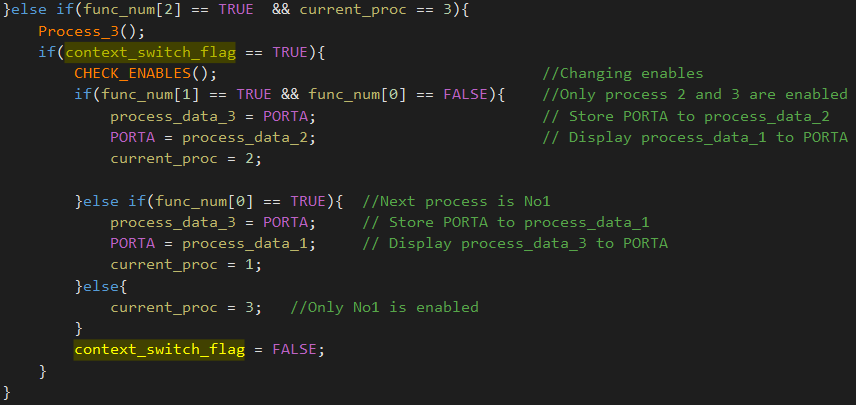
\includegraphics[height=3.5cm, width=\linewidth]{./results/lab8_main_proc_3.png}
			\caption{C code for Process 3 context switching}
		\end{subfigure}
	\end{figure}
	
	\pagebreak
	\noindent
	Οι interrupt handler των δύο TIMER0 και TIMER1, είναι πολύ απλοί και αυτό που κάνουν είναι να θέτουν TRUE κάποια flags για το πότε να αλλάξει μια διεργασία το PORTA και πότε γίνεται το context switch μεταξύ των διεργασιών. Για τον handler του USART, αυτό που κάνουμε είναι κα ελέγχουμε αν ήρθε κάποιο enable ή disable κάποιας διεργασίας και αναλόγως.\\
	
	\noindent
	Όσον αφορά το USART, αυτό που κάνουμε είναι να διαβάζουμε χαρακτήρα χαρακτήρα την κάθε εντολή. Στην περίπτωση που λαμβάνουμε κάποια εντολή Sx<CR><LF>, αποθηκεύουμε στο (x-1)-bit του byte func\_enable την τιμή "1". Αν πχ έρθει η τιμή 1, κάνουμε set το bit 0 στο "1", αν έρθει 2 κάνουμε το bit 1 set "1" και, τέλος, αν έρθει 3 κάνουμε το bit 2 set στον "1". \\
	
	 \noindent
	 Aντίθετα, στην περίπτωση που έρθει κάποιο Qx<CR><LF>, αποθηκεύουμε στο (x-1)-bit του byte \\ func\_enable την τιμή "0". Έτσι, αν έρθει η τιμή 1, κάνουμε clear το bit 0, αν έρθει 2 κάνουμε clear το bit 1 και αν έρθει 3 κάνουμε clear το bit 2. \\
	\begin{figure}[h!]
		\centering
		\begin{subfigure}[t]{0.5\textwidth}
			\centering
			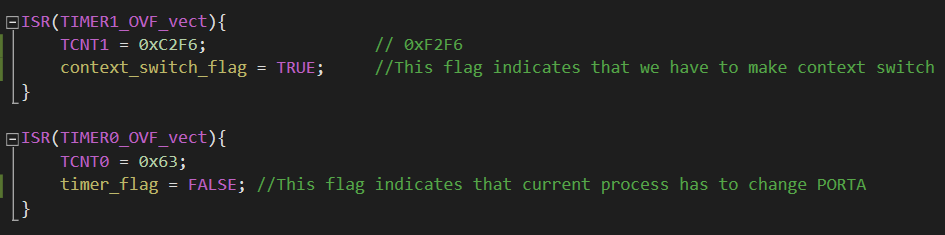
\includegraphics[height=4cm, width=\linewidth]{./results/lab8_timer_handlers.png}
			\caption{C code for TIMER0/TIMER1 OVF interrupt handlers}
		\end{subfigure}%
		~
		\begin{subfigure}[t]{0.5\textwidth}
			\centering
			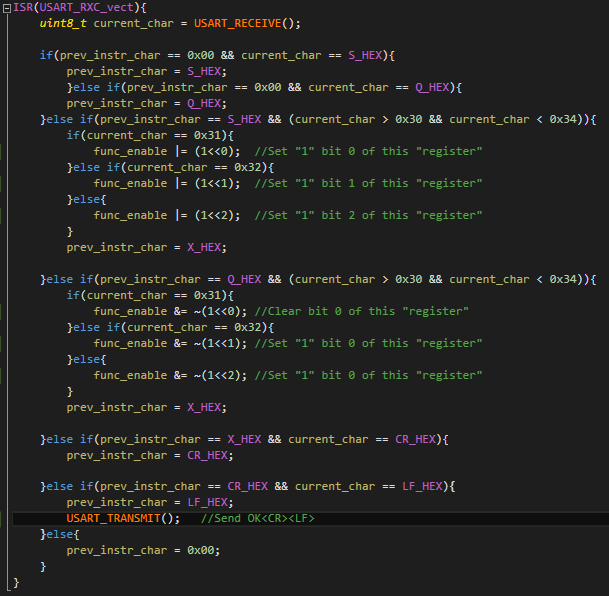
\includegraphics[height=4cm, width=\linewidth]{./results/lab8_usart_handler.png}
			\caption{C code for USART RXC interrupt handler}
		\end{subfigure}
	\end{figure}
	
	\pagebreak
	\noindent
	\textbf{Προσομοίωση Αποτελεσμάτων} \\
	\noindent
	Aρχικά, στην εικόνα (a) βλέπουμε ότι λαμβάνουμε σωστά από τη USART την εντολή S2<CR><LF> και αποθηκεύονται σωστά οι τιμές των enable τόσο στο array func\_num όσο και στη μεταβλητή func\_enable. Στο array αποθηκεύεται η τιμή "0x01" στη θέση 1, ενώ στη μεταβλητή η τιμή είναι "0x02" που σημαίνει οτι το bit 1 είναι "1". Oμοίως, στην εικόνα (b) βλέπουμε ότι βλέπουμε ότι λαμβάνουμε το S1<CR><LF> και στο array αποθηκεύεται η τιμή "0x01" στη θέση 2, ενώ στη μεταβλητή η τιμή είναι "0x03" που σημαίνει οτι το bit 0 και 1 είναι "1". Τέλος, βλέπουμε και η εντολή S3<CR><LF> λαμβάνεται σωστά και το array έχει την τιμή "0x01" σε όλες τις θέσεις του και η μεταβλητή έχει την τιμή "0x07" που σημαίνει ότι τα bit 0,1 και 2 είναι "1".\\
	
	\begin{figure}[h!]
		\centering
		\begin{subfigure}[t]{0.5\textwidth}
			\centering
			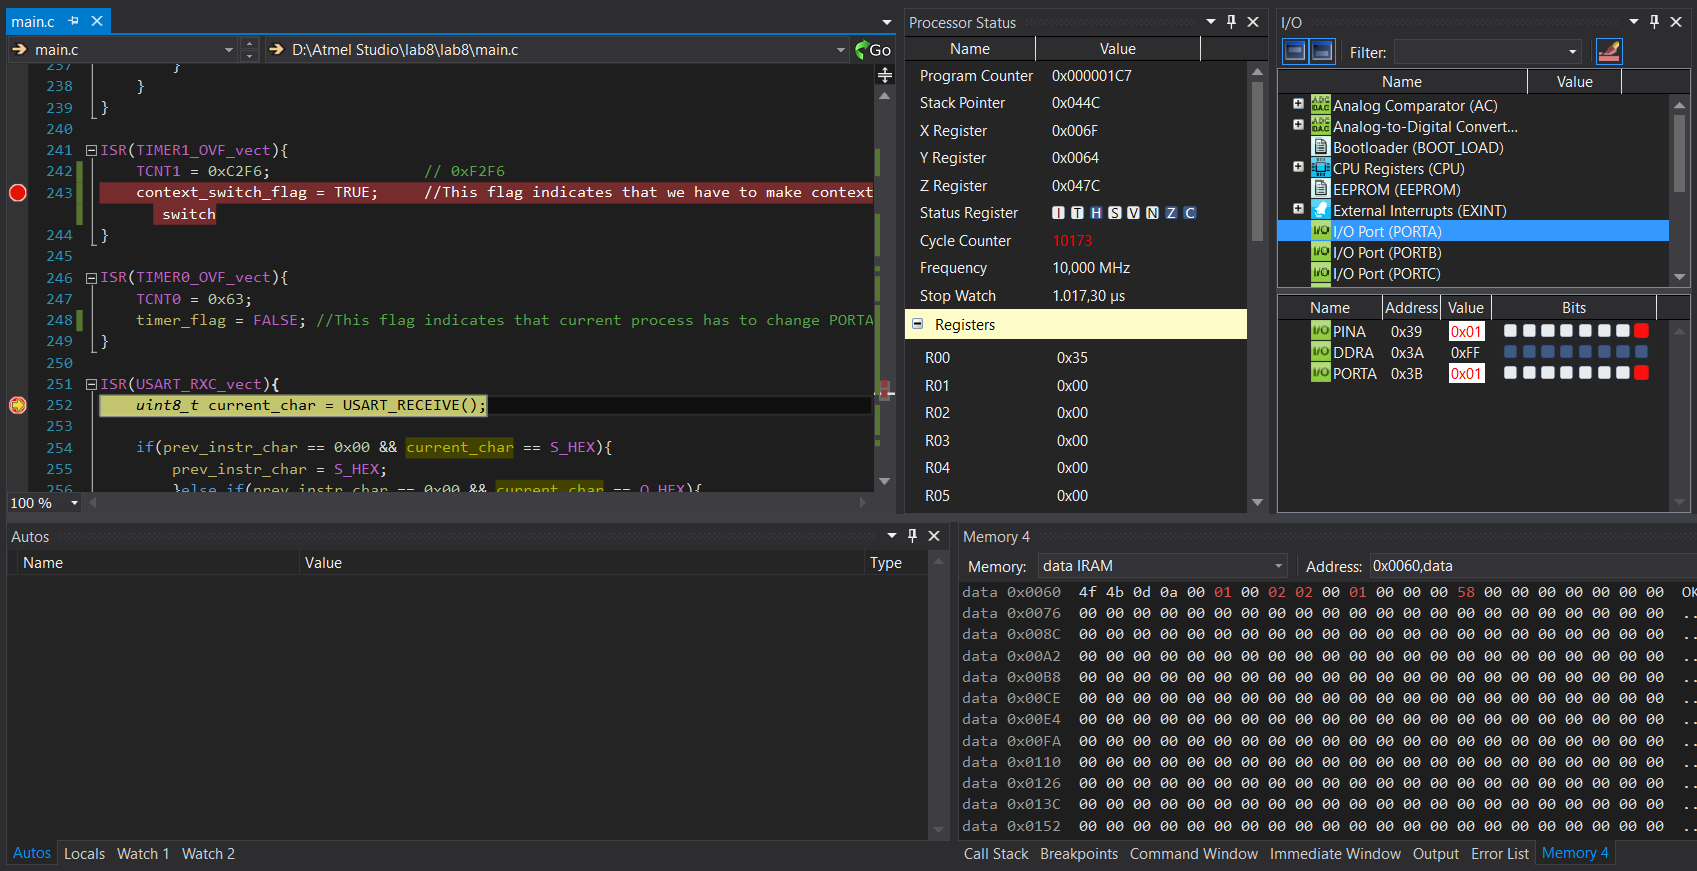
\includegraphics[height=3cm,width=\linewidth]{./results/lab8_sim_proc_2.png}
			\caption{Results from Αtmel Studio 7 - Only Process 2 is enabled}
		\end{subfigure}%
		~
		\begin{subfigure}[t]{0.5\textwidth}
			\centering
			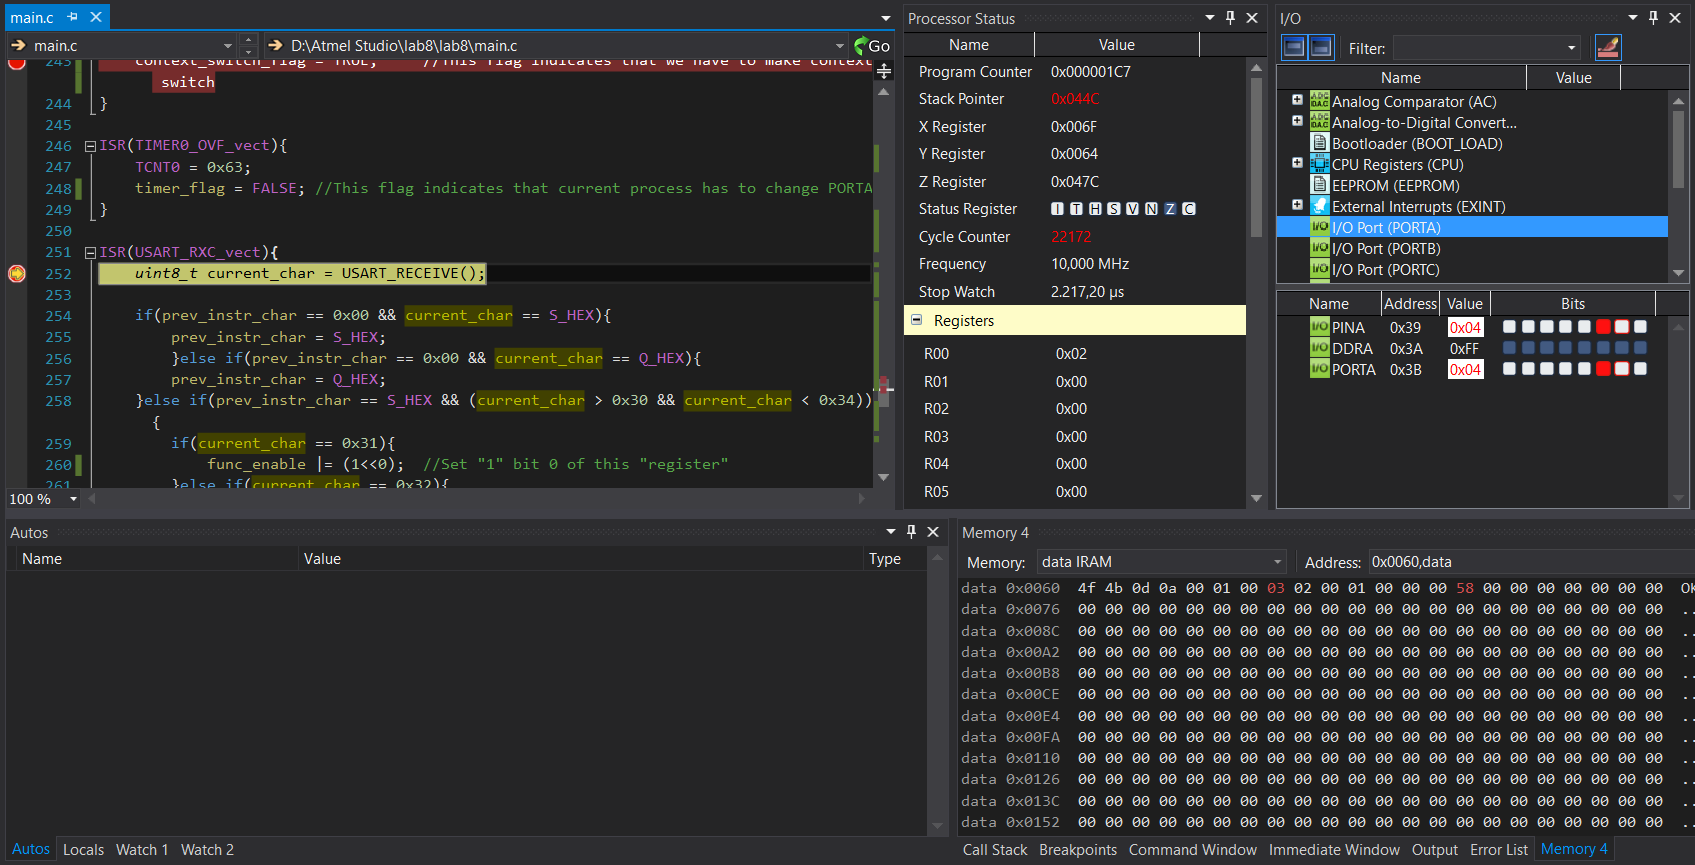
\includegraphics[height=3cm,width=\linewidth]{./results/lab8_sim_proc_1.png}
			\caption{Results from Αtmel Studio 7 - Process 1 is enabled }
		\end{subfigure}
		
		\begin{subfigure}[t]{0.5\textwidth}
			\centering
			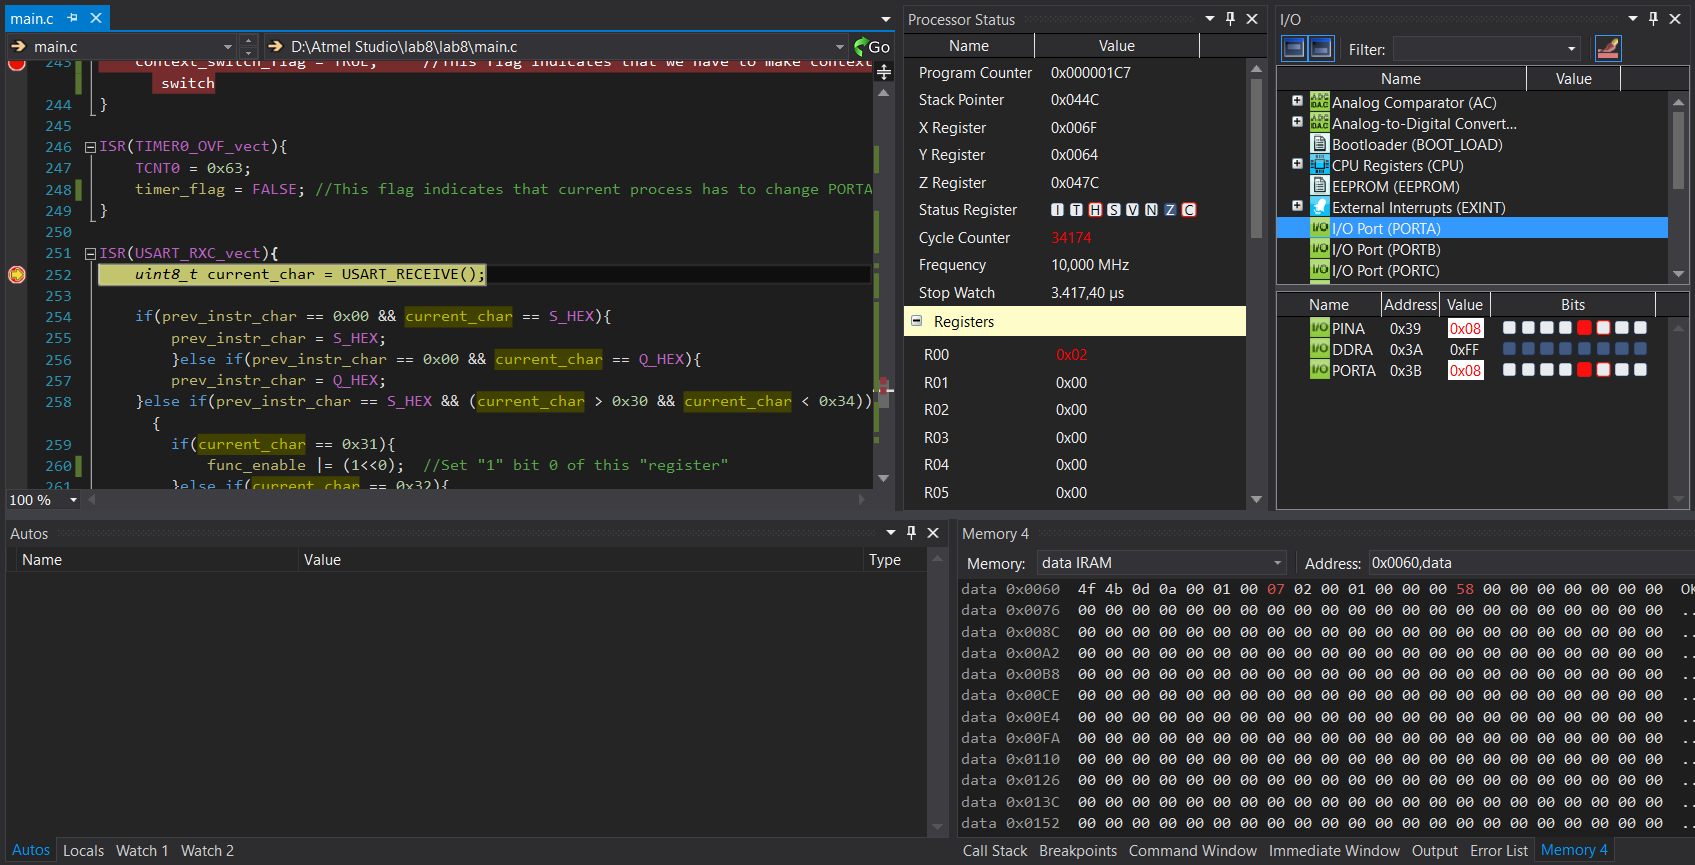
\includegraphics[height=3cm,width=\linewidth]{./results/lab8_sim_proc_3.png}
			\caption{Results from Αtmel Studio 7 - Process 3 is enabled}
		\end{subfigure}
	\end{figure}

	\noindent
	Στις παρακάτω εικόνες βλέπουμε το context switch μεταξύ των διεργασιών. Στην εικόνα (a) φαίνεται ότι τα δεδομένα που είχε επεξεργαστεί το Process 2 στο PORTA, έχουν αποθηκευτεί στη μνήμη. Παράλληλα, βλέπουμε ότι έχει έρθει και ο TIMER1 και το timeslice της διεργασίας 3 τελείωσε και πρέπει να γίνει context switch μεταξύ της 3 και της 1. Στην επόμενη εικόνα (b), φαίνεται ότι τα δεδομένα του Process 3 αποηθηκεύτηκαν και αυτά στη μνήμη, ενώ ήρθε και πάλι ο TIMER1, αυτή τη φορά για το context switch μεταξύ της 1 και της 2. Τέλος, όπως φαίνεται στην εικόνα (c), και τα δεδομένα του Process 1 αποθηκεύτηκαν στη μνήμη και γίνεται context switch μεταξύ της 2 και της 3 για δεύτερη φορά.\\
	\begin{figure}[h!]
		\centering
		\begin{subfigure}[t]{0.5\textwidth}
			\centering
			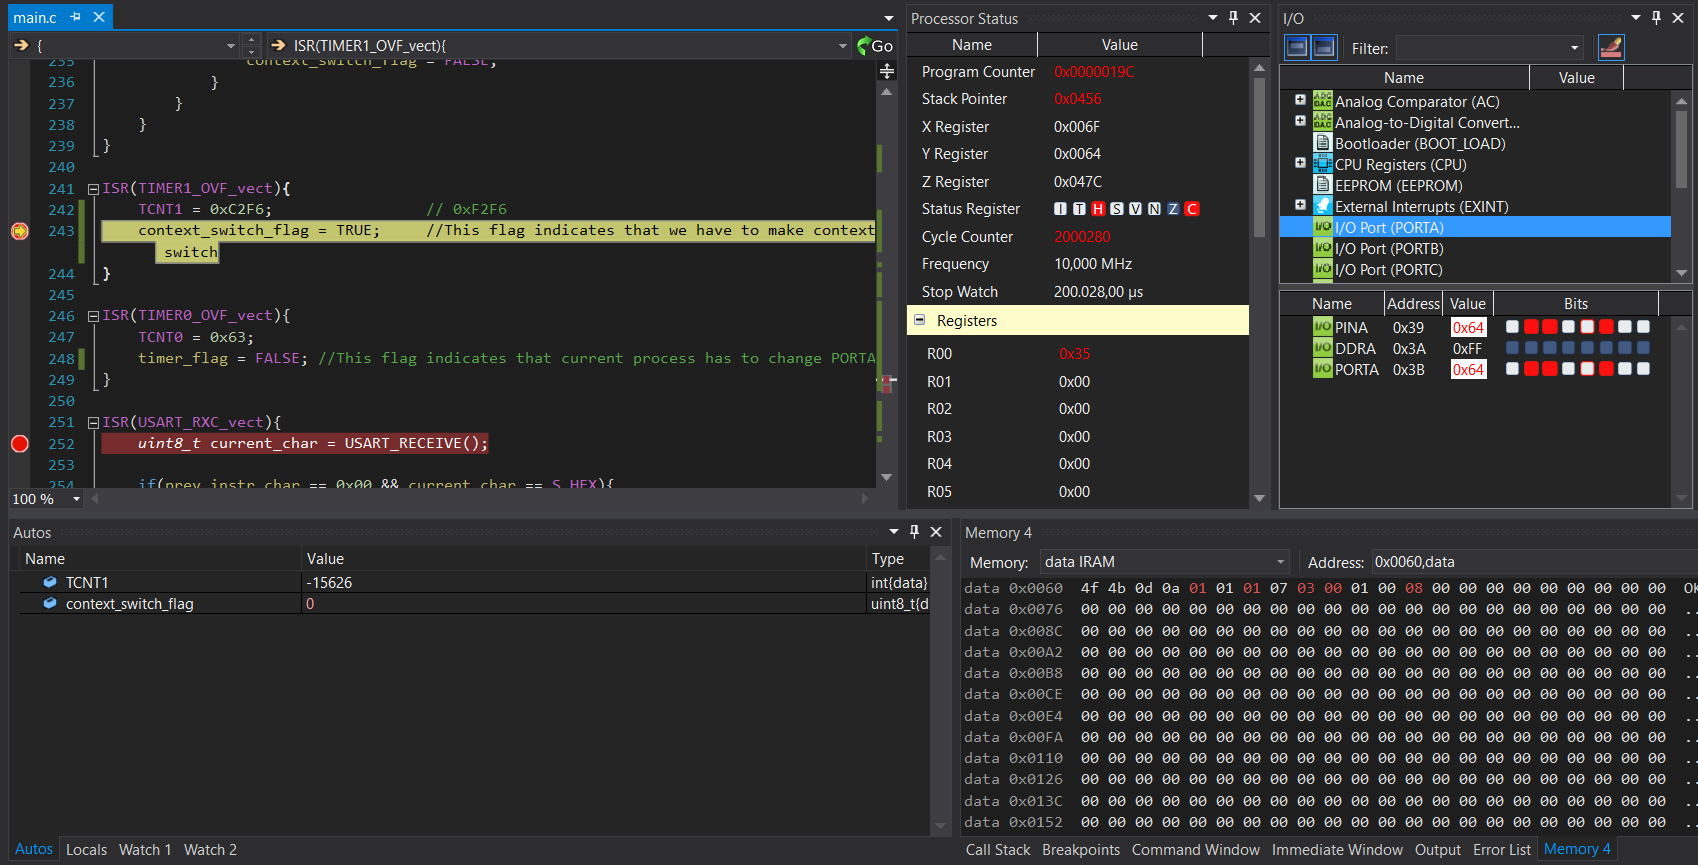
\includegraphics[height=3cm,width=\linewidth]{./results/lab8_sim_cs_2_3.png}
			\caption{Results from Αtmel Studio 7 - Context Switch between Process 2 and 3}
		\end{subfigure}%
		~
		\begin{subfigure}[t]{0.5\textwidth}
			\centering
			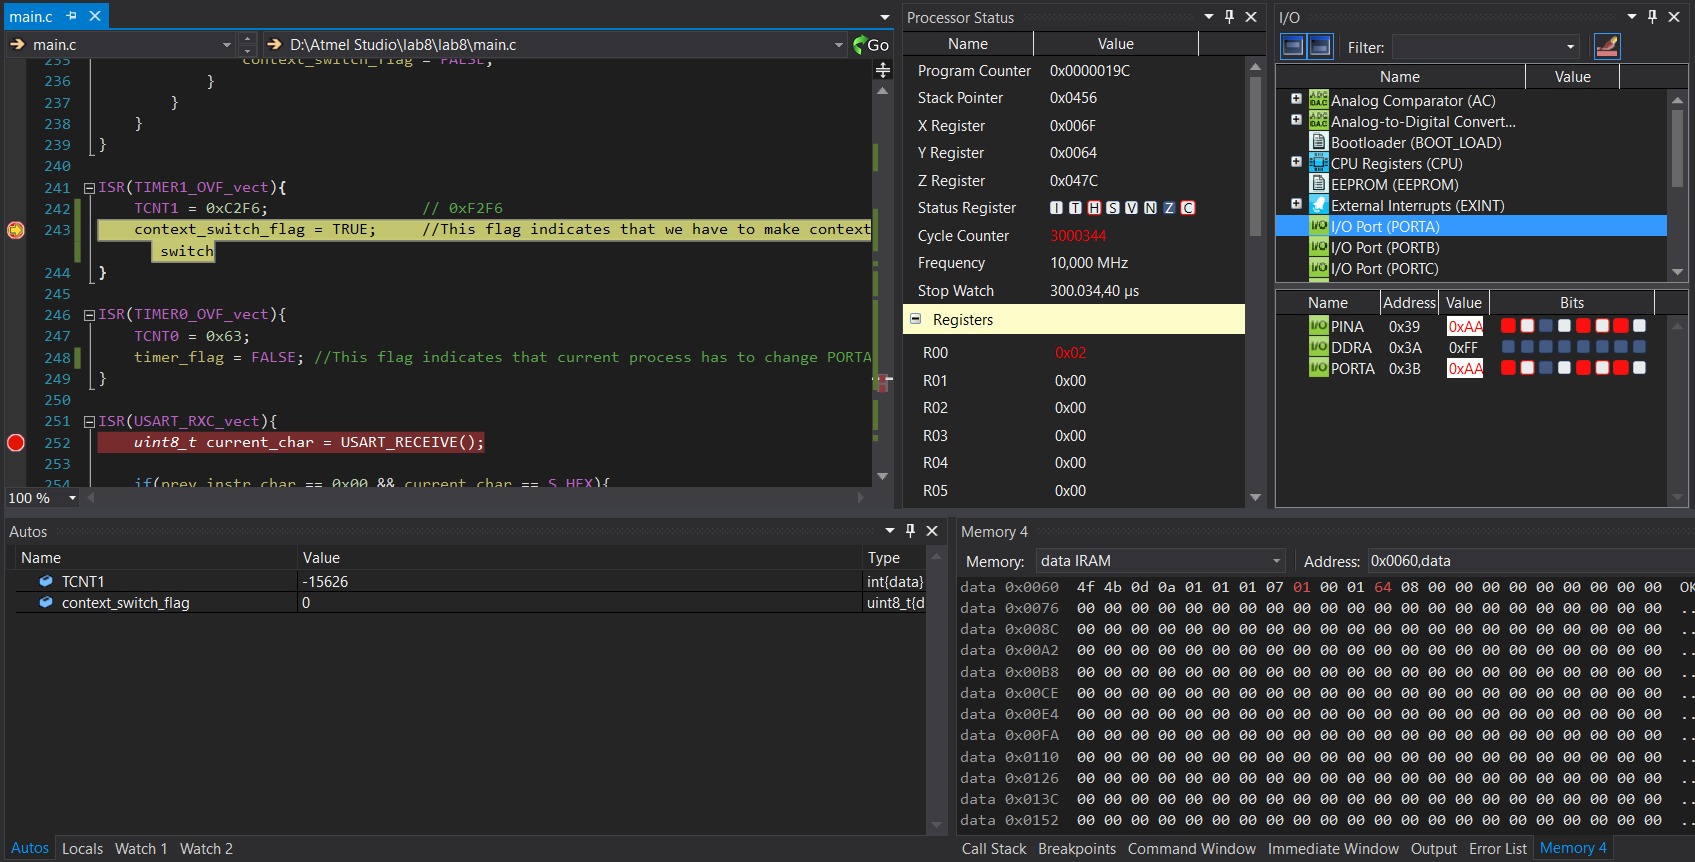
\includegraphics[height=3cm,width=\linewidth]{./results/lab8_sim_cs_3_1.png}
			\caption{Results from Αtmel Studio 7 - Context Switch between Process 3 and 1}
		\end{subfigure}
		
		\begin{subfigure}[t]{0.5\textwidth}
			\centering
			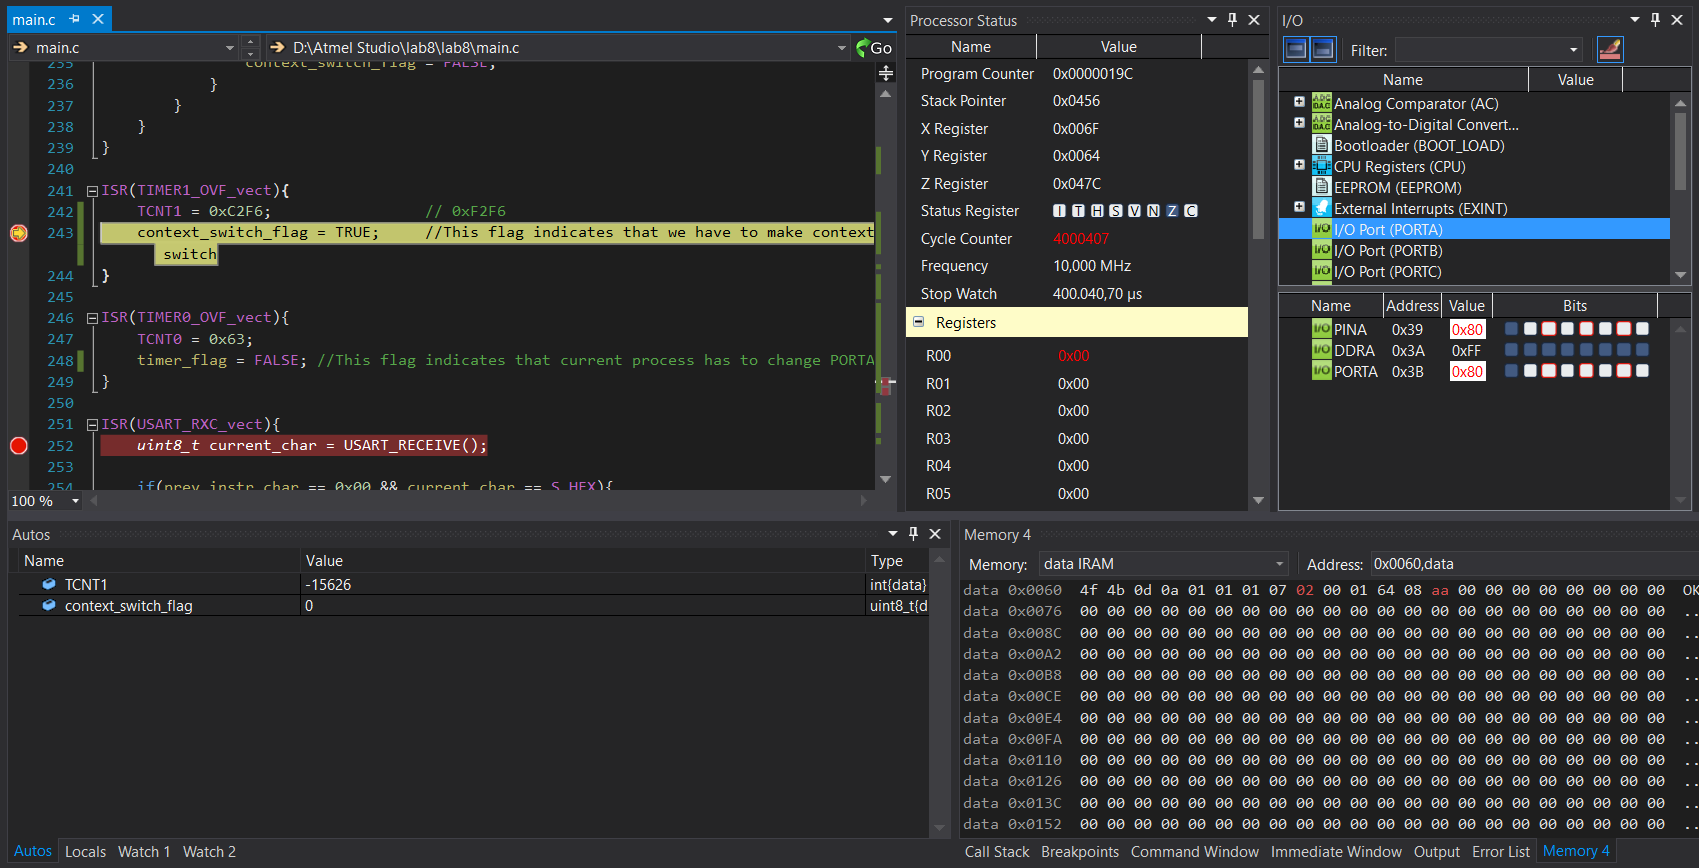
\includegraphics[height=3cm,width=\linewidth]{./results/lab8_sim_cs_1_2.png}
			\caption{Results from Αtmel Studio 7 - Context Switch between Process 1 and 2}
		\end{subfigure}
	\end{figure}

	\pagebreak
	\noindent
	Στην εικόνα (a) φαίνεται ότι μετά την εντολή Q2<CR><LF> η διεργασία 2 απενεργοποιείται και τα δεδομένα της καθαρίζονται από τη μνήμη. Επίσης, βλέπουμε ότι μετά το context switch μεταξύ της 2 και της 3 έγινε σωστά και η 2 έγινε quit αμέσως μετά το context switch. Eπίσης, στην ίδια εικόνα φαίνεται ότι είμαστε στην περίοδο που το timeslice της 1 τελείωσε και τα δεδομένα της θα αποθηκευτούν στη μνήμη. Στην εικόνα (b) βλέπουμε ότι γίνεται σωστά και η εντολή Q1<CR><LF> και η μοναδική διεργασία που έμεινε είναι η 3. Σε αυτή την περίπτωση αφού είναι η μοναδική διεργασία που αλλάζει το PORTA, δε χρειάζεται να αποθηκεύσουμε κάτι στη μνήμη εφόσον δεν γίνεται κάποιο context switch.\\
	
	\begin{figure}[h!]
		\centering
		\begin{subfigure}[t]{0.5\textwidth}
			\centering
			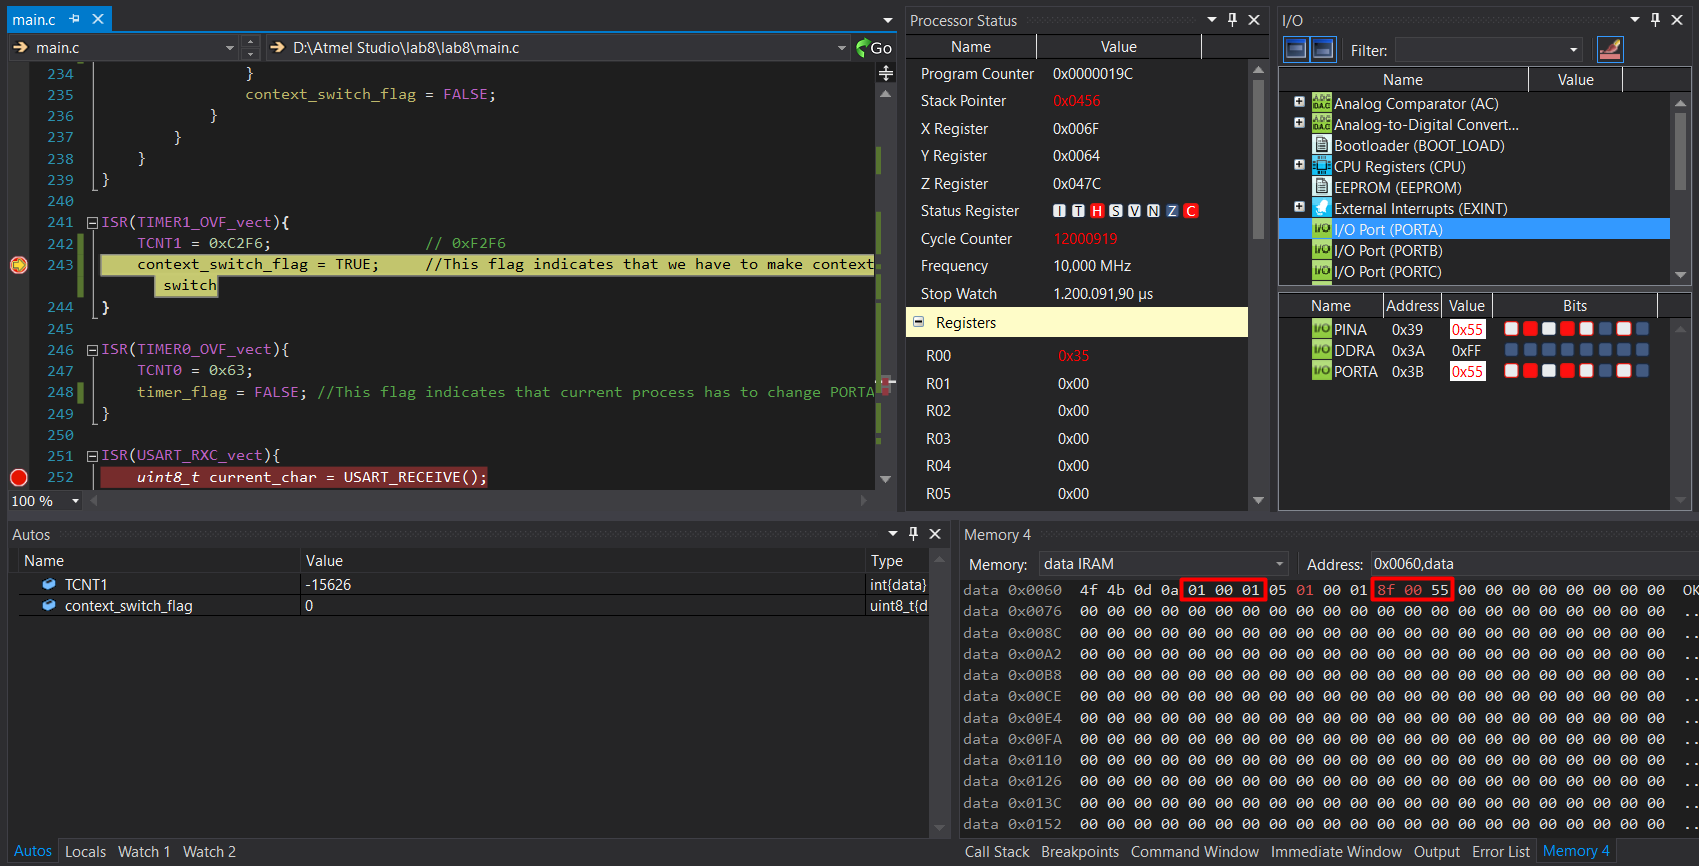
\includegraphics[height=3.5cm,width=\linewidth]{./results/lab8_sim_q2_cs_3_1.png}
			\caption{Results from Αtmel Studio 7 - Quit process 2}
		\end{subfigure}%
		~
		\begin{subfigure}[t]{0.5\textwidth}
			\centering
			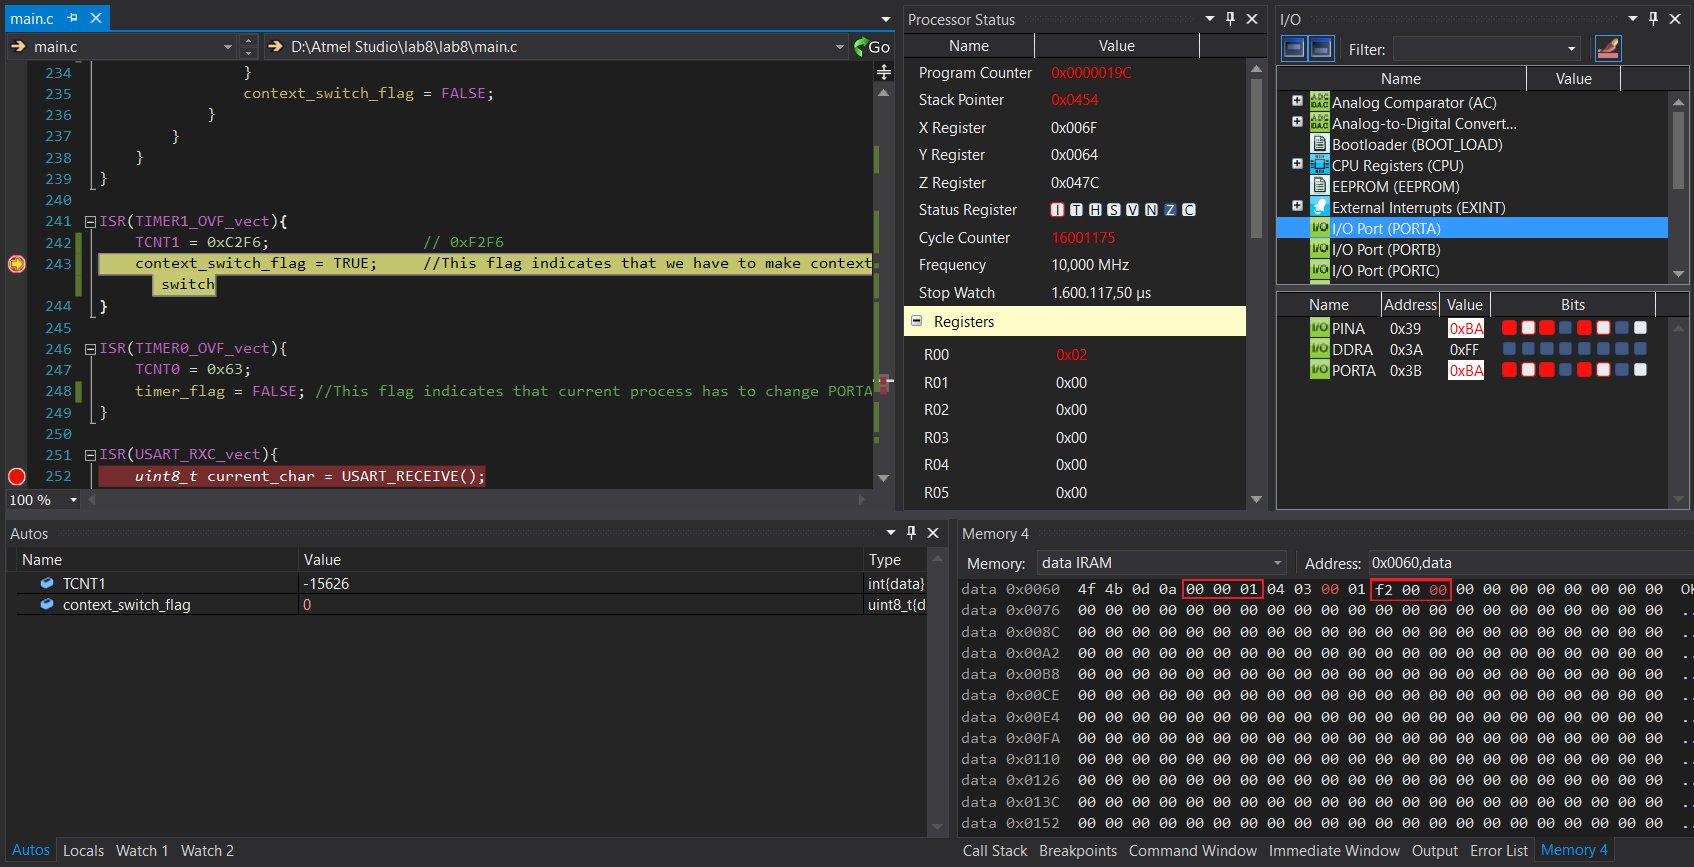
\includegraphics[height=3.5cm,width=\linewidth]{./results/lab8_sim_q1_cs_1_3.png}
			\caption{Results from Αtmel Studio 7 - Quit process 1}
		\end{subfigure}
	\end{figure}

	\noindent
	Στις παρακάτω εικόνες, κάνουμε ξανά start την διεργασία 1 την οποία είχαμε σταματήσει. όπως φαίνεται στην εικόνα (a) η εντολή start εκτελέστηκε σωστά και oι ενεργές διεργασίες είναι η 1 και η 3. Επίσης, φαίνεται ότι στο προηγούμενο timeslice τα δεδομένα της διεργασίας 1 αποθηκεύτηκαν στη μνήμη, ενώ ήρθε ο TIMER1, καθώς το timeslice της 3 τελείωσε. Στην τελευταία εικόνα βλέπουμε το αντίθετο, δηλαδή στο προηγούμενο timeslice τα δεδομένα της διεργασίας 3 αποθηκεύτηκαν στη μνήμη, ενώ ήρθε ο TIMER1, καθώς το timeslice της 1 τελείωσε και συνεπώς πρέπει να γίνει context switch μεταξύ των διεργασιών.
	
	\begin{figure}[h!]
	\centering
	\begin{subfigure}[t]{0.5\textwidth}
		\centering
		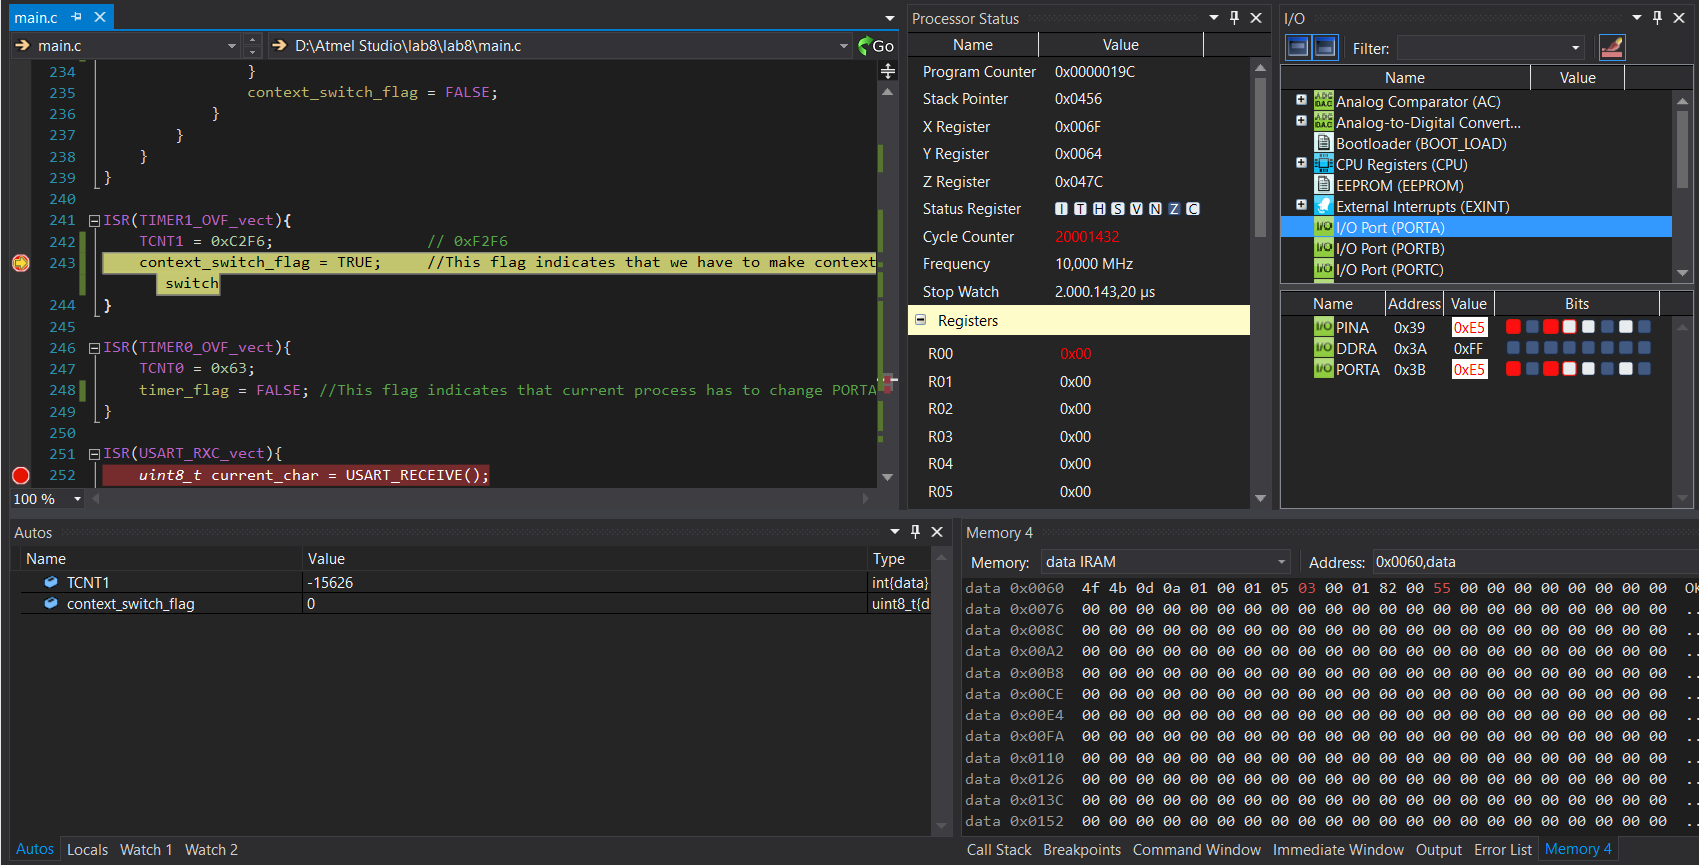
\includegraphics[height=3.5cm,width=\linewidth]{./results/lab8_sim_s1_cs_3_1.png}
		\caption{Results from Αtmel Studio 7 - Start process 1 }
	\end{subfigure}%
	~
	\begin{subfigure}[t]{0.5\textwidth}
		\centering
		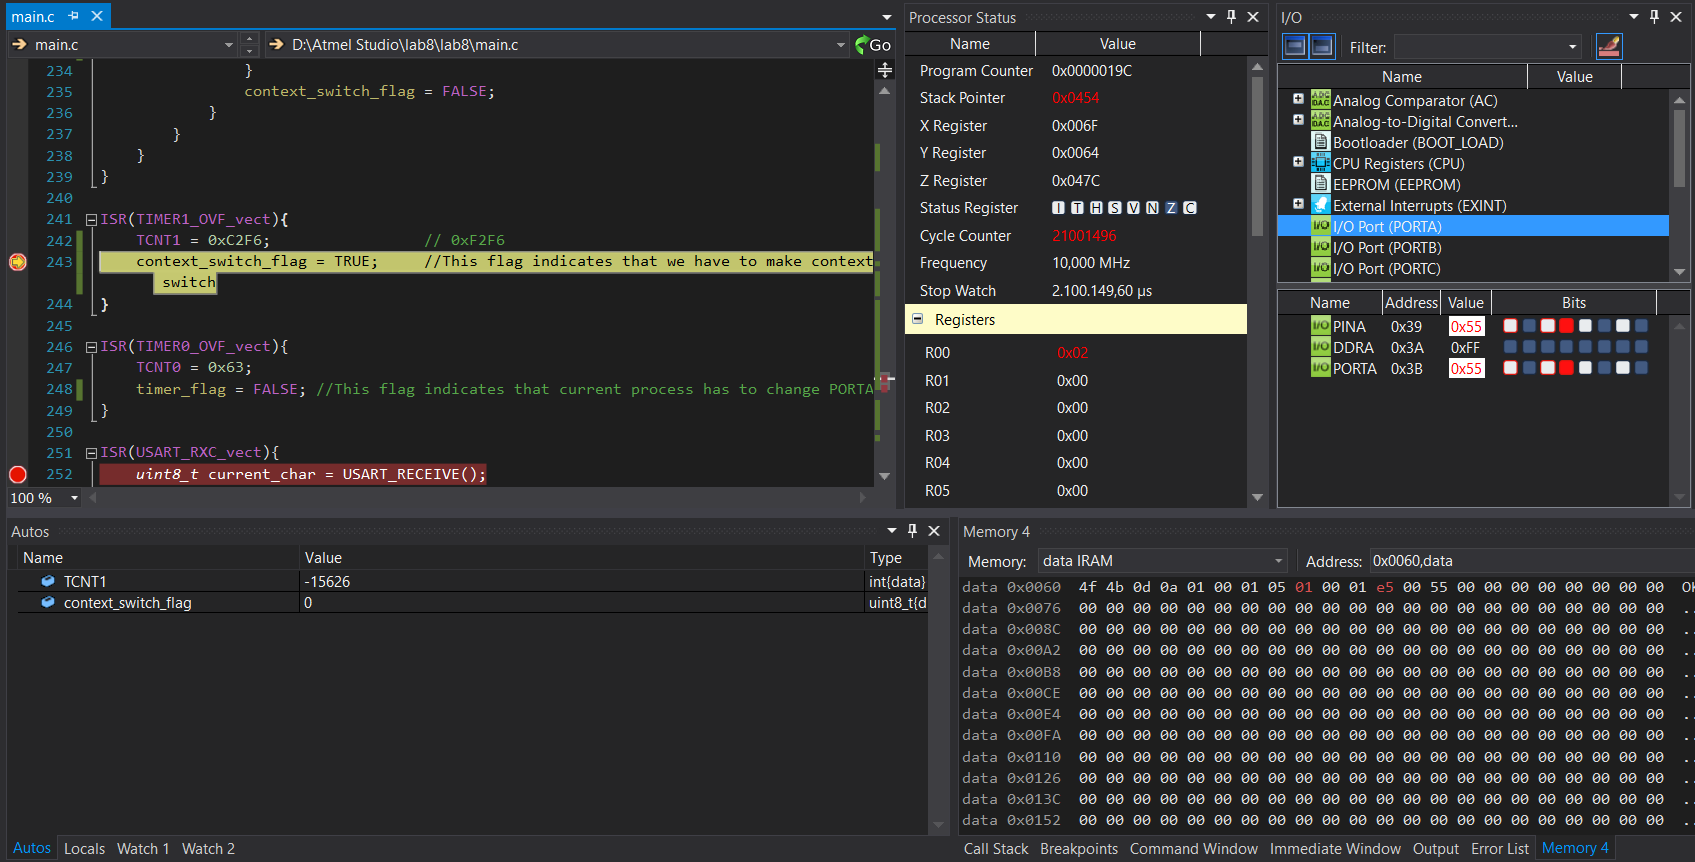
\includegraphics[height=3.5cm,width=\linewidth]{./results/lab8_sim_s1_cs_1_3.png}
		\caption{Results from Αtmel Studio 7 - Context Switch between Process 3 and 1}
	\end{subfigure}
\end{figure}
\end{document}
